\chapter{Desarrollo}
\label{hardware}

\section{Búsqueda de información}
\label{busqueda_informacion}

El primer paso es identificar el hardware del que disponemo en la fábrica con ayuda de las fotos tomadas:
    \begin{figure}[H]
            \centering
            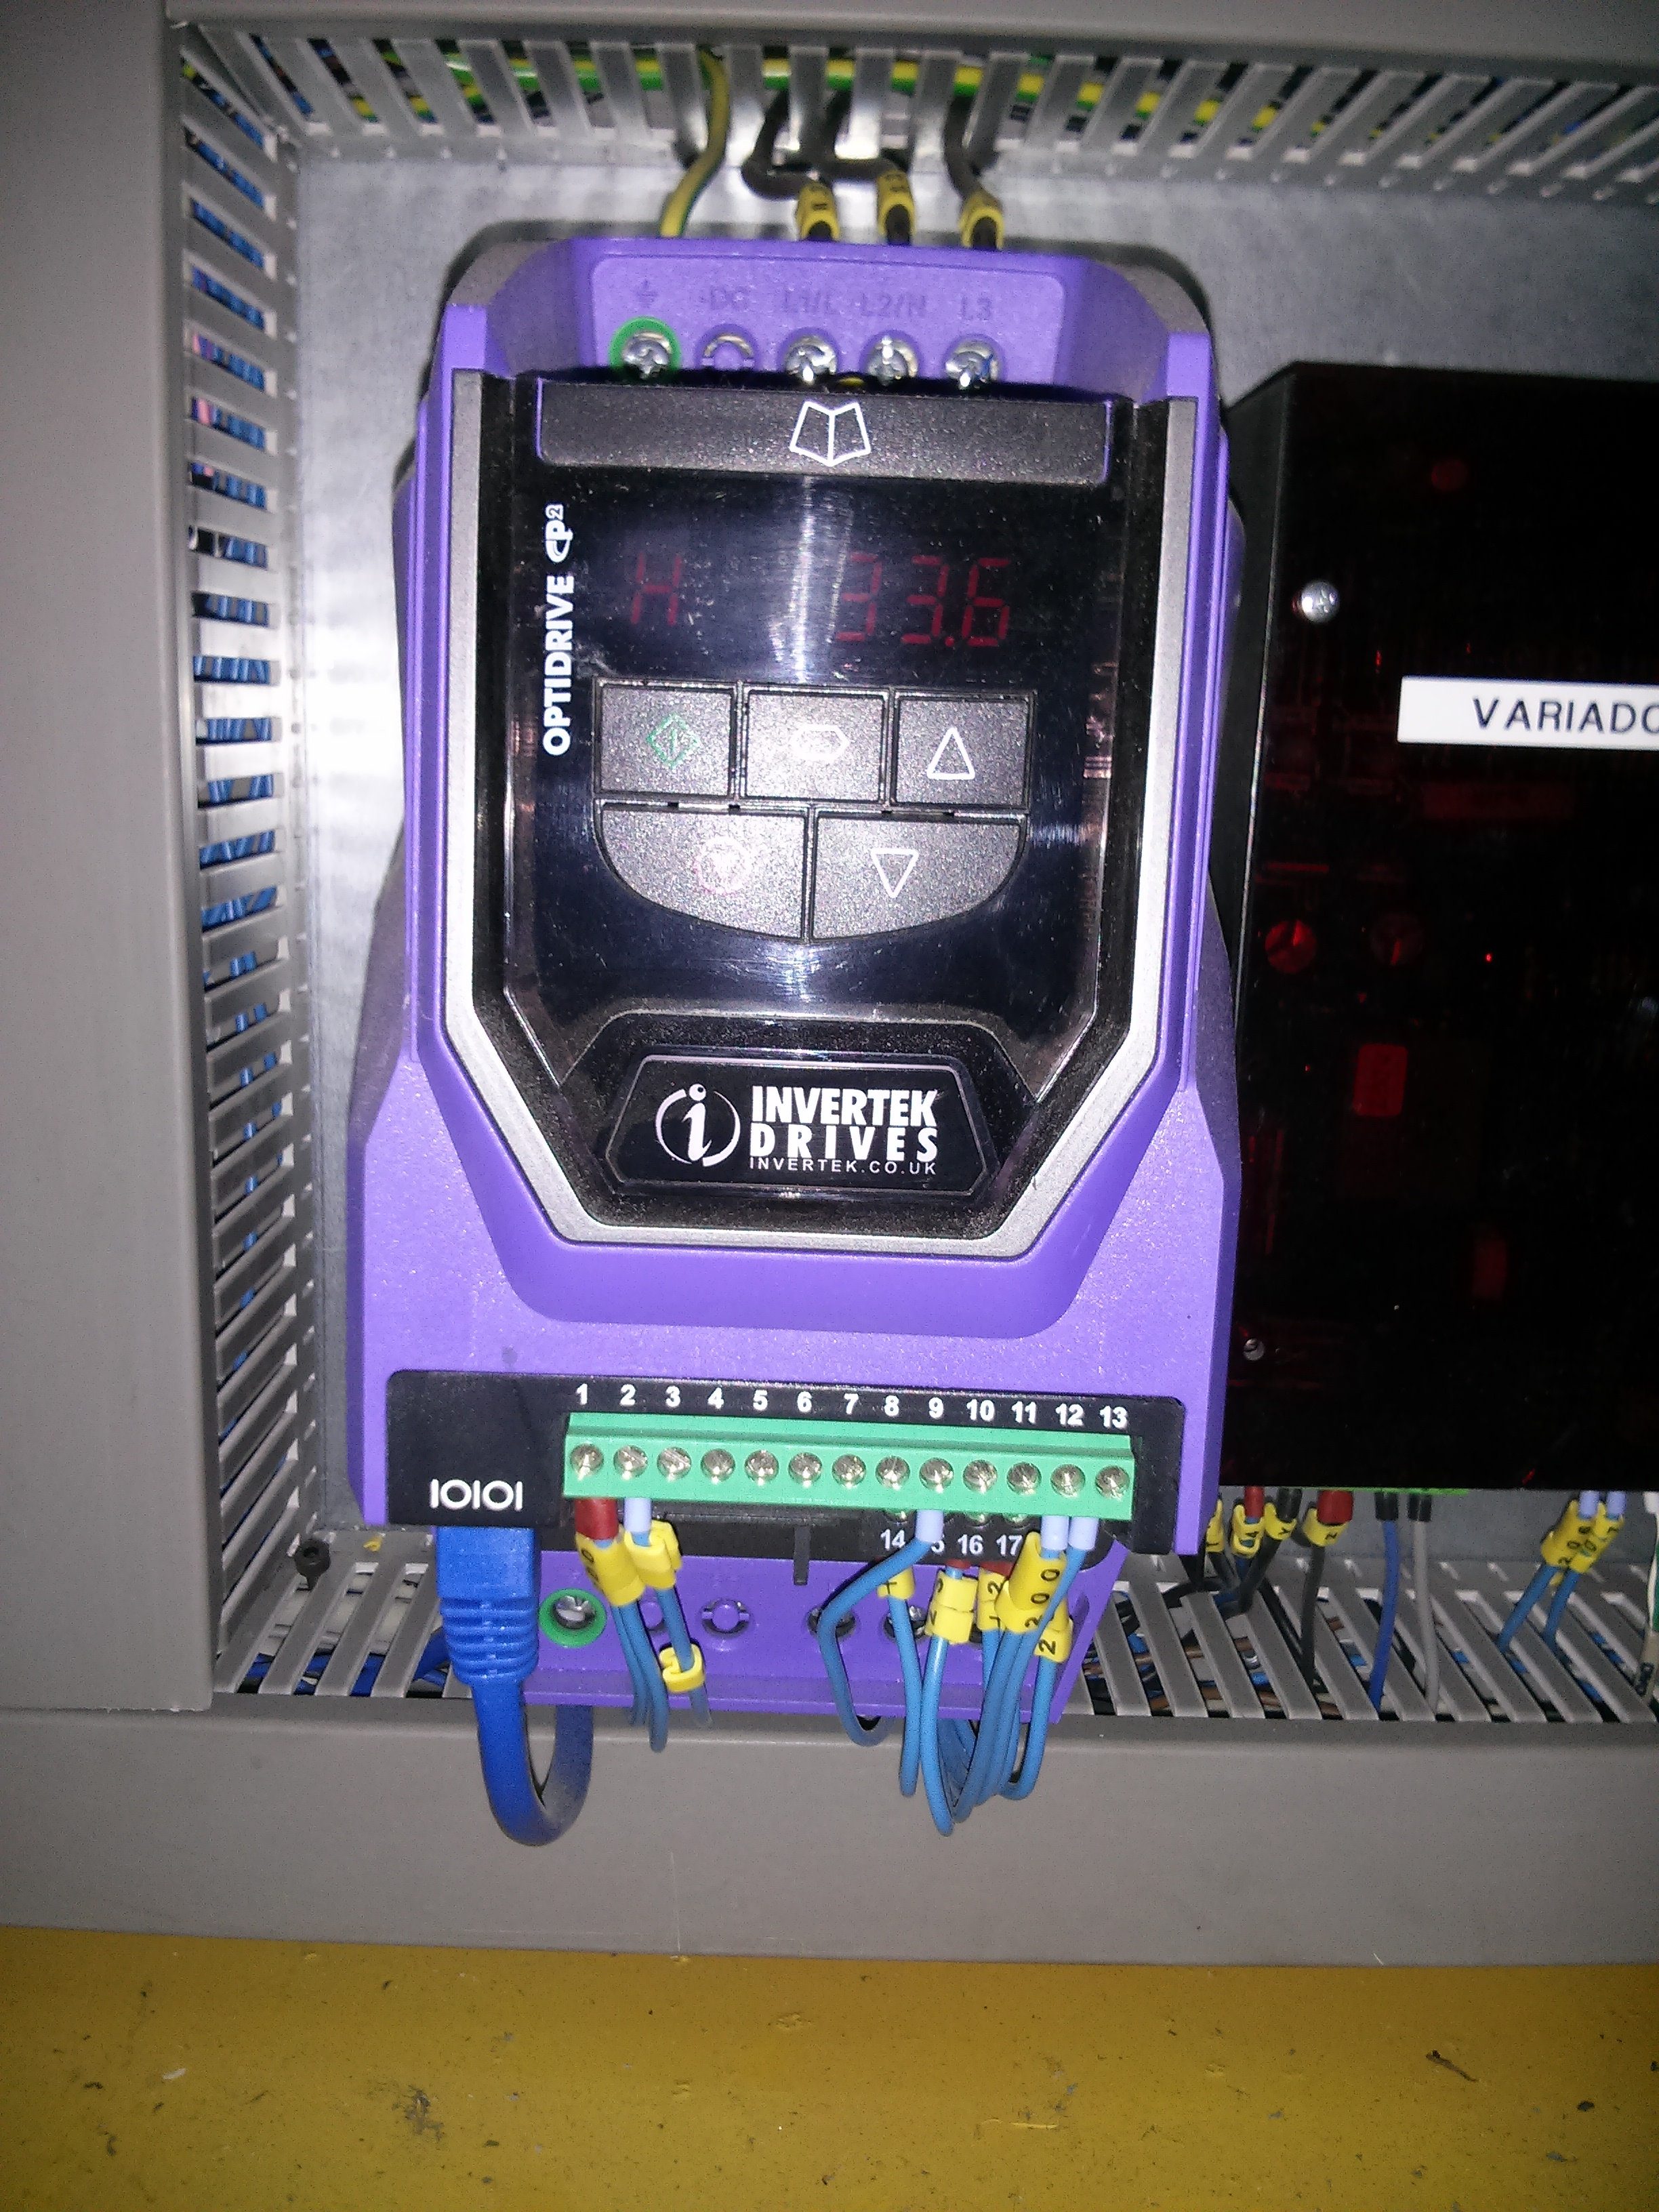
\includegraphics[width=0.4\textwidth]{images/huesca/IMG_20141216_174810.jpg}
            \caption{Variador Optidrive}
            \label{fig:hardware_variador}
    \end{figure}

    \begin{figure}[H]
            \centering
            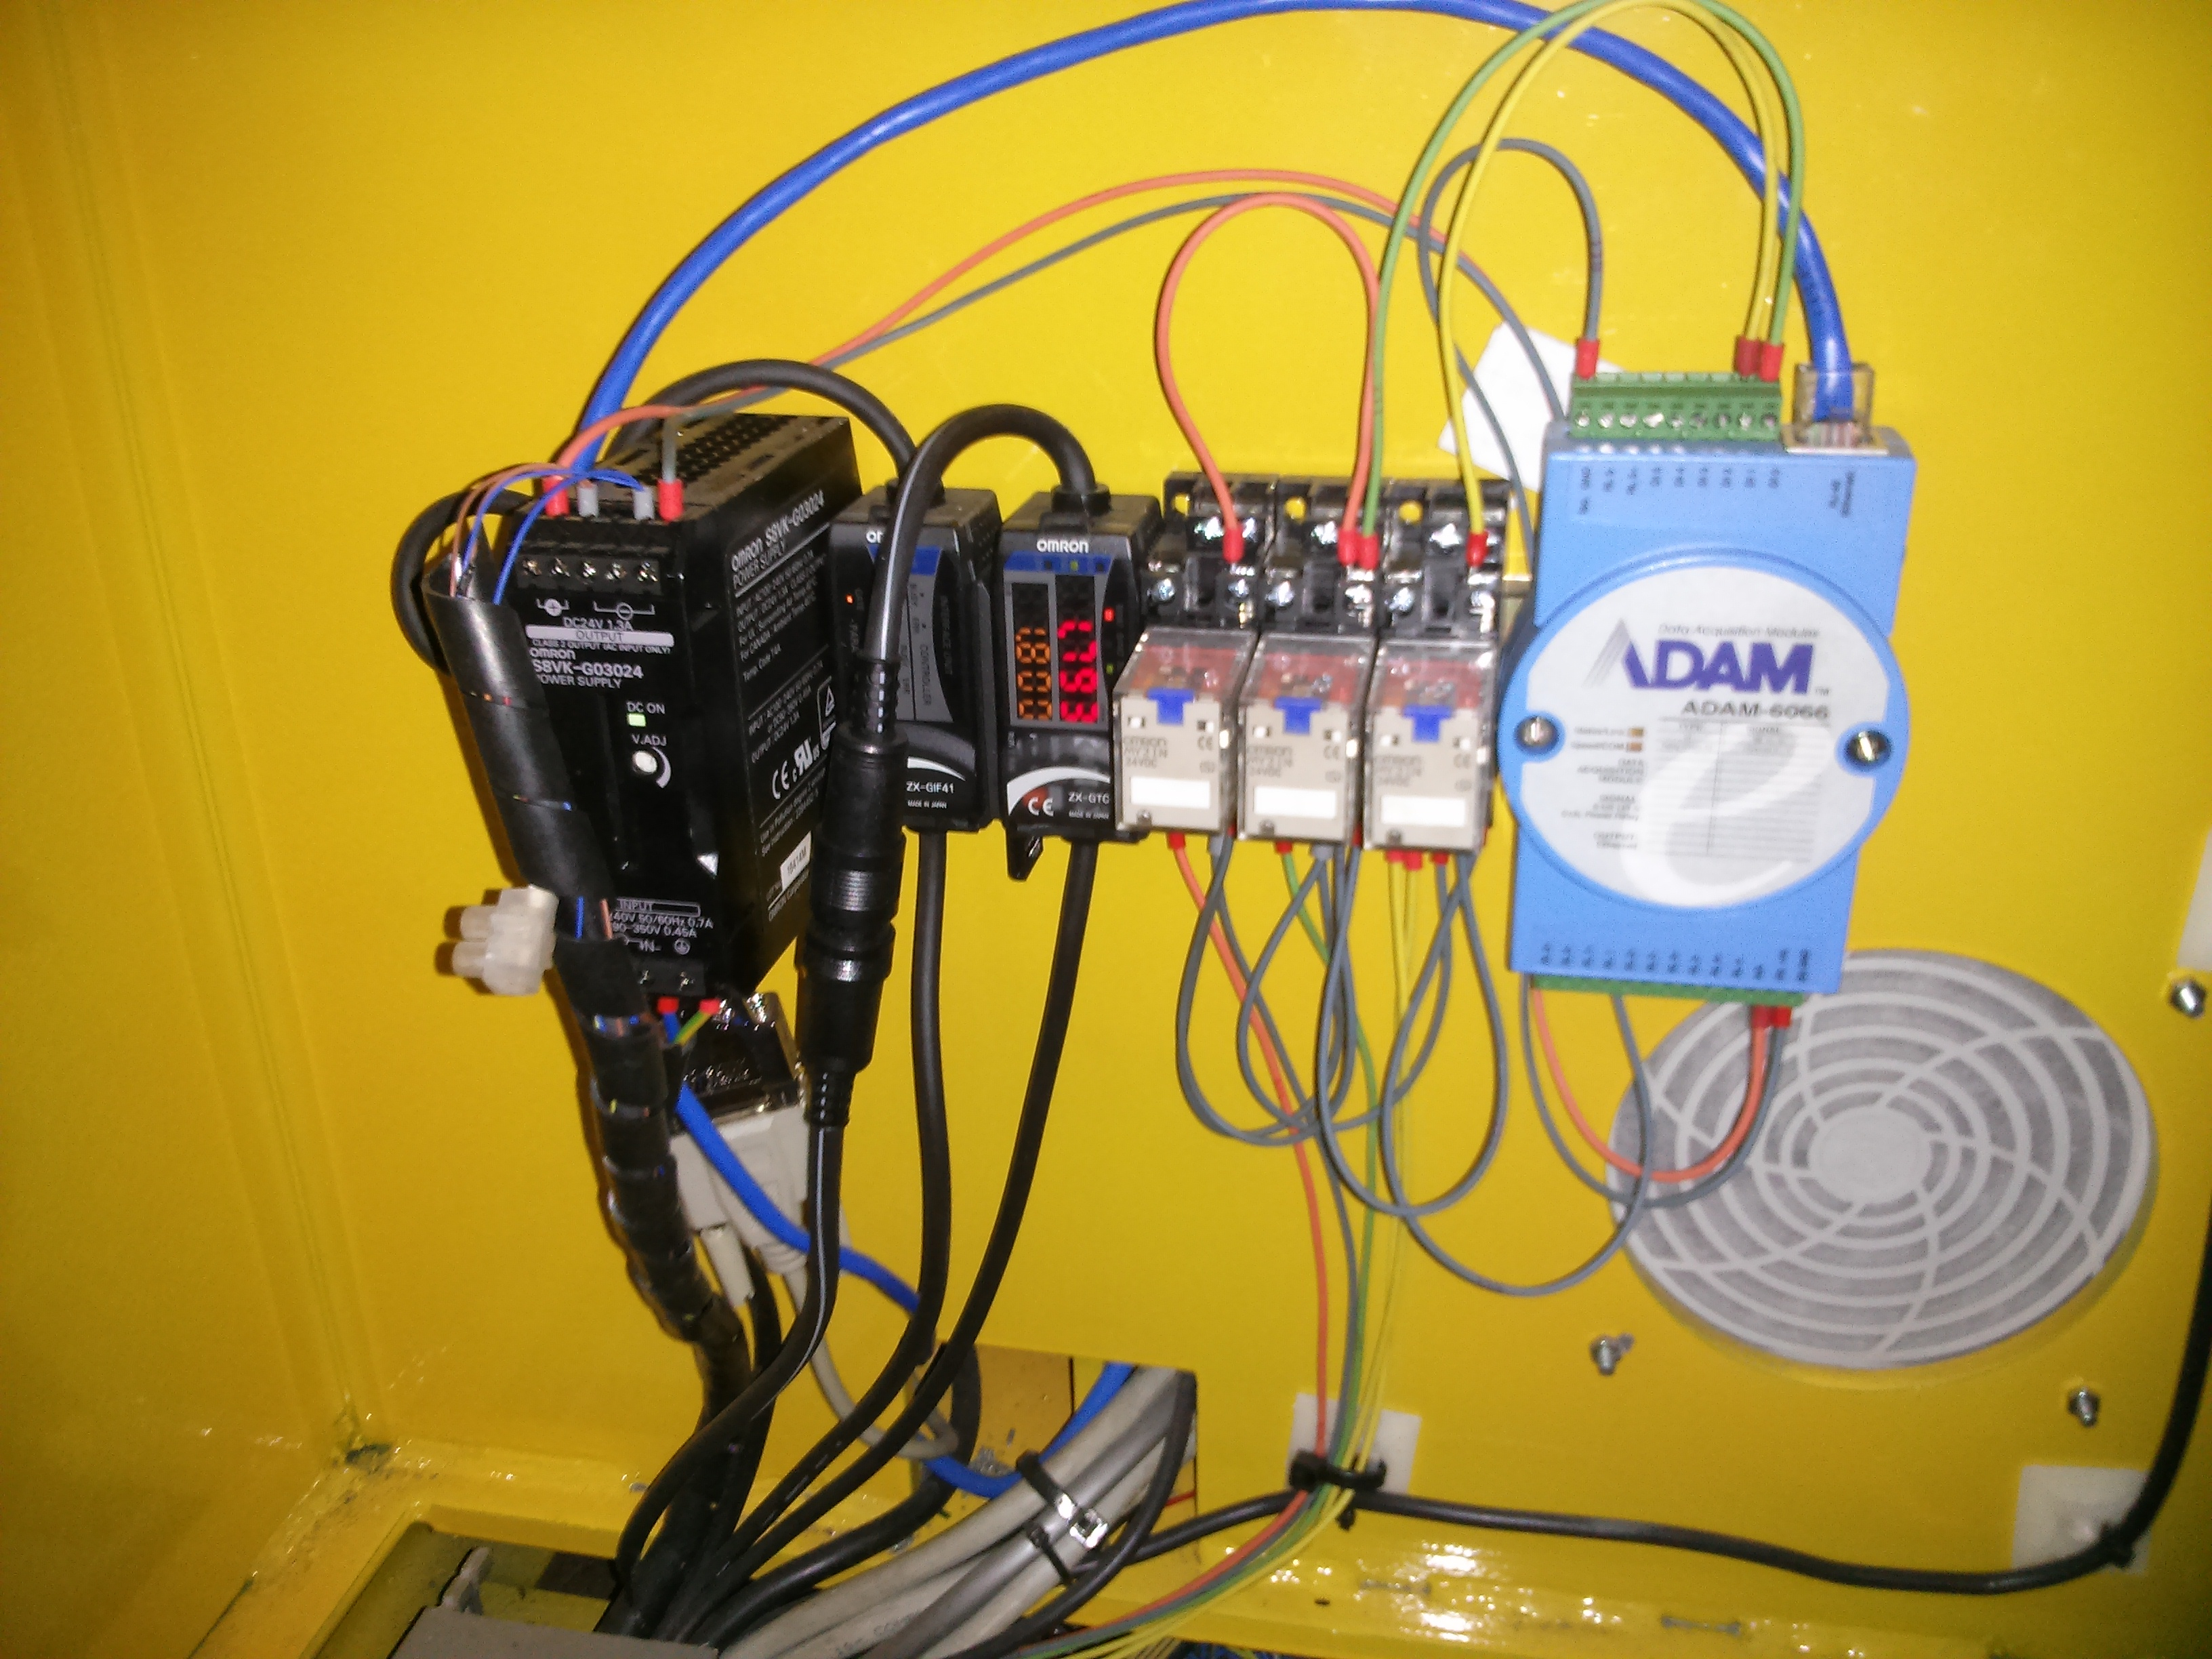
\includegraphics[width=0.4\textwidth]{images/huesca/IMG_20141216_174824.jpg}
            \caption{Sensor de diámetro y perifería}
            \label{fig:hardware_diametro}
    \end{figure}

    \begin{figure}[H]
            \centering
            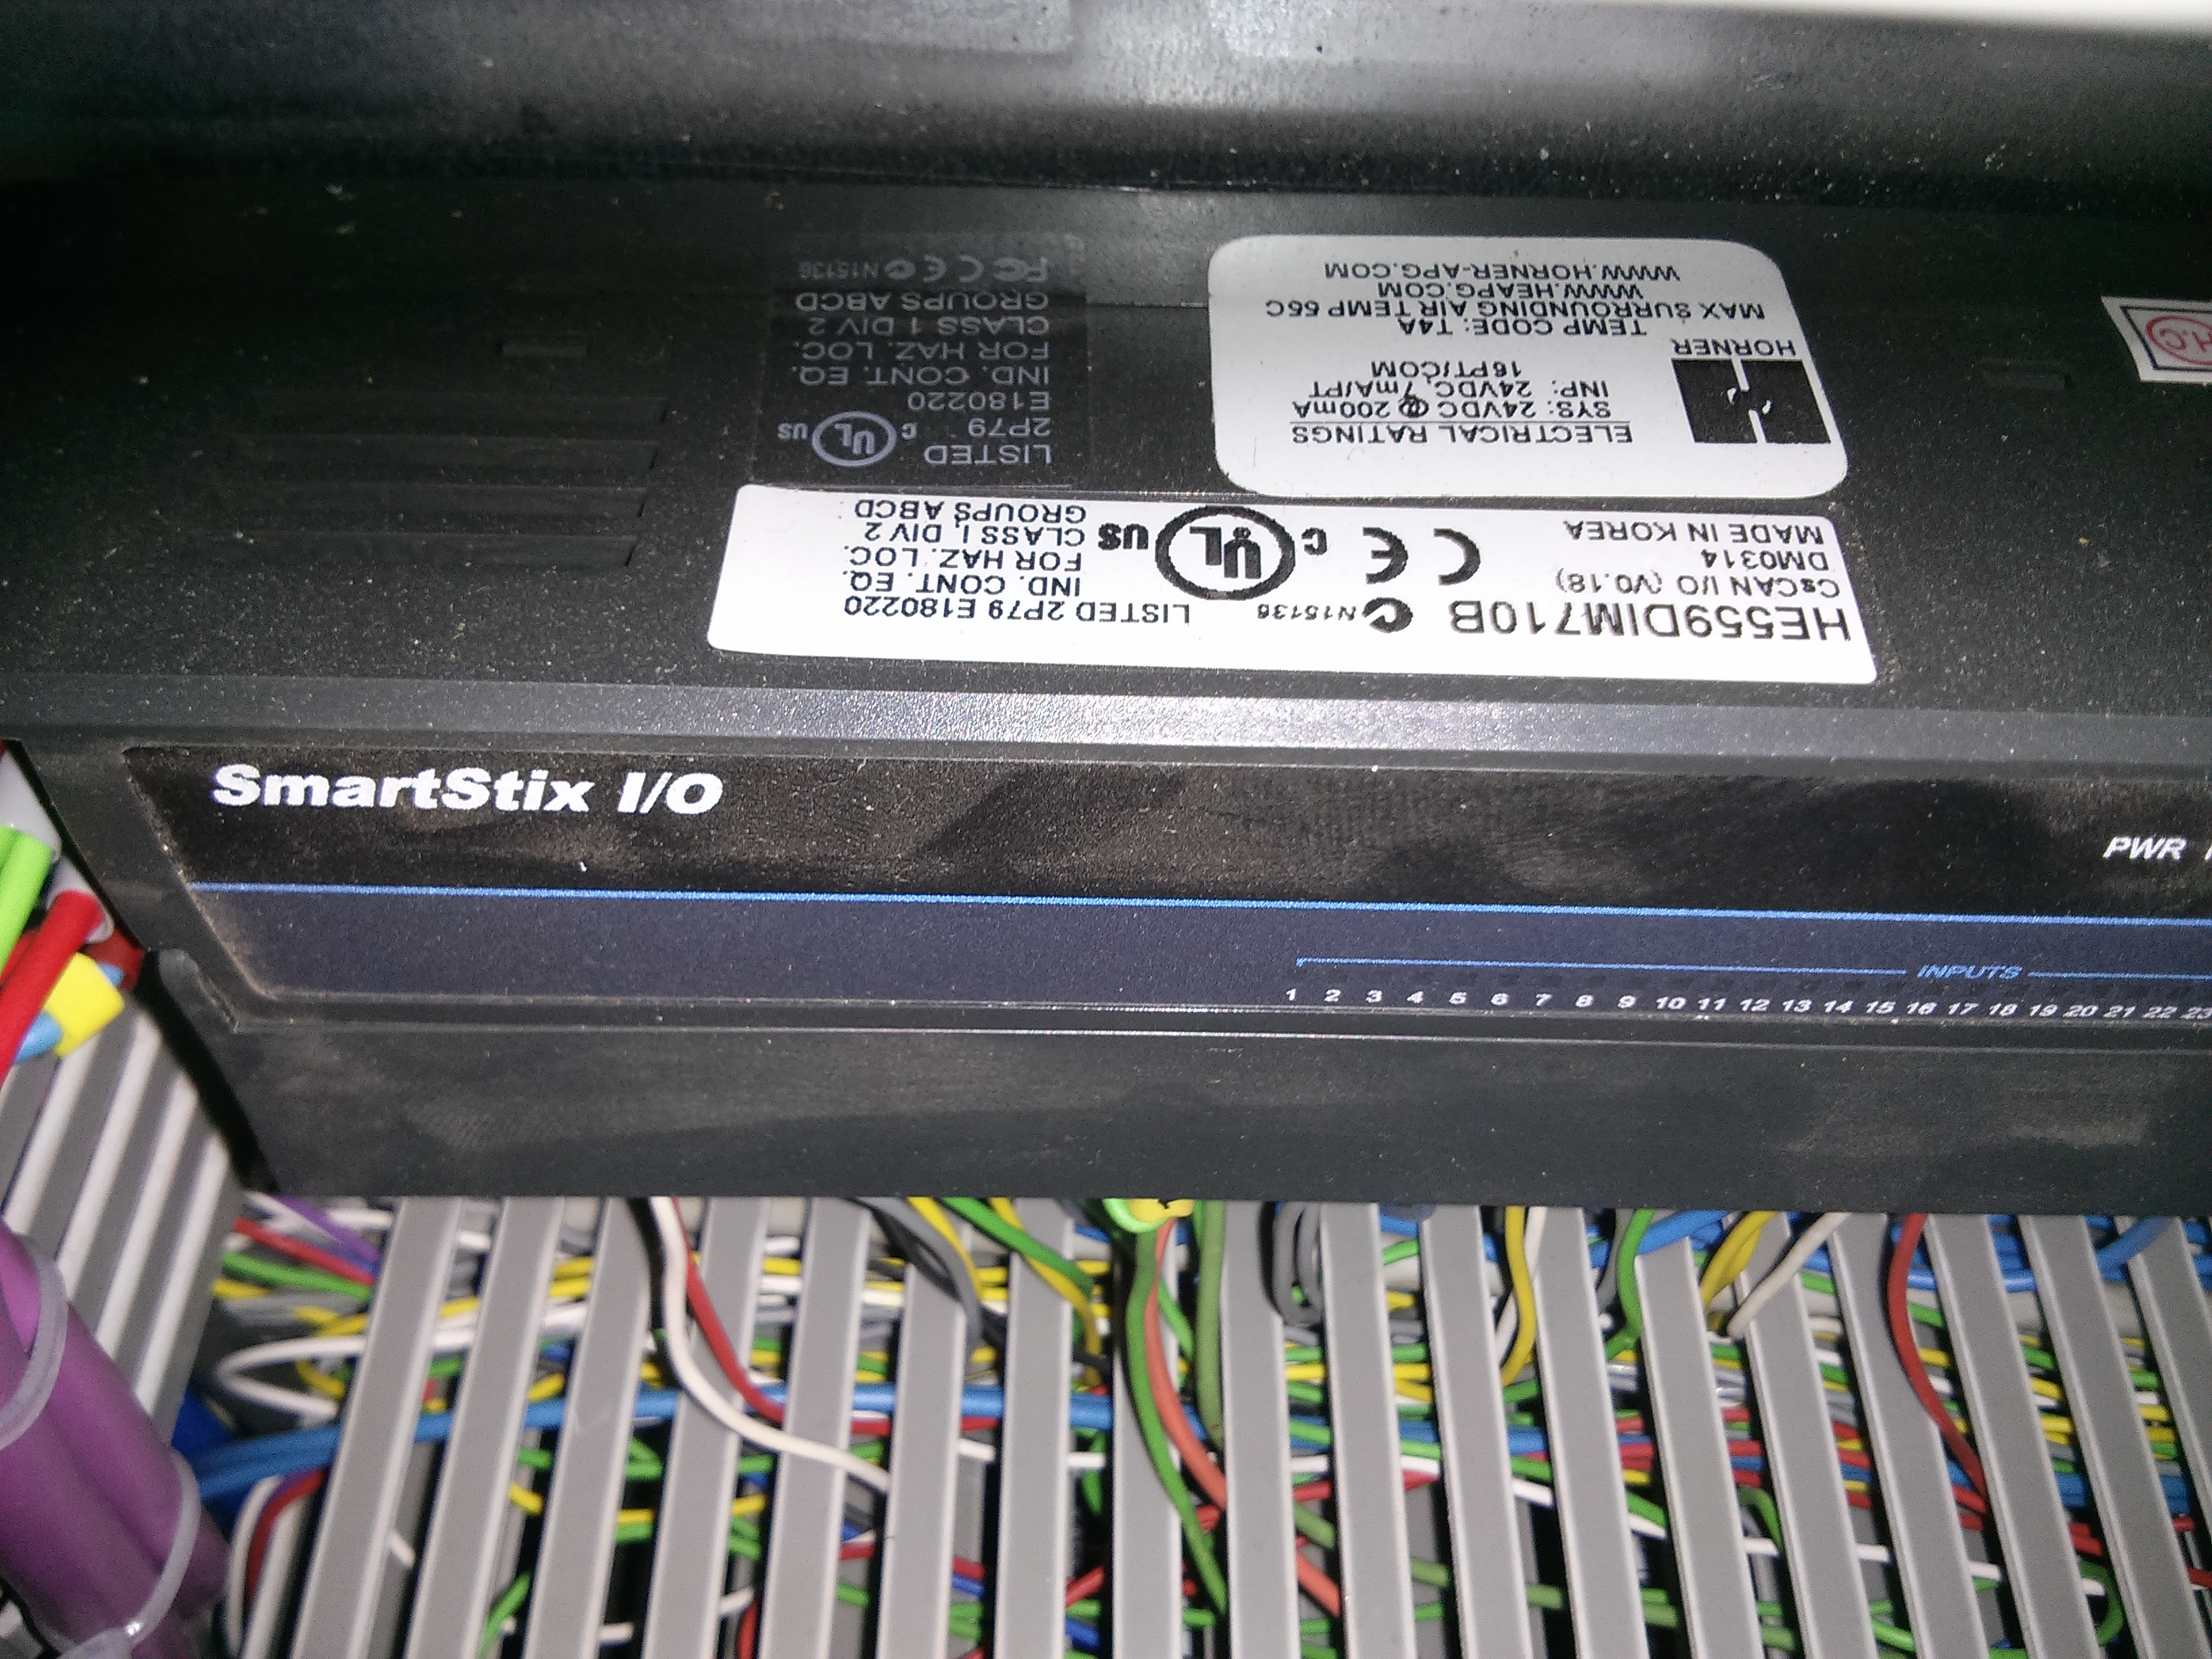
\includegraphics[width=0.4\textwidth]{images/huesca/IMG_20141216_174925.jpg}
            \caption{Perifería distribuida}
            \label{fig:hardware_periferia}
    \end{figure}

    \begin{figure}[H]
            \centering
            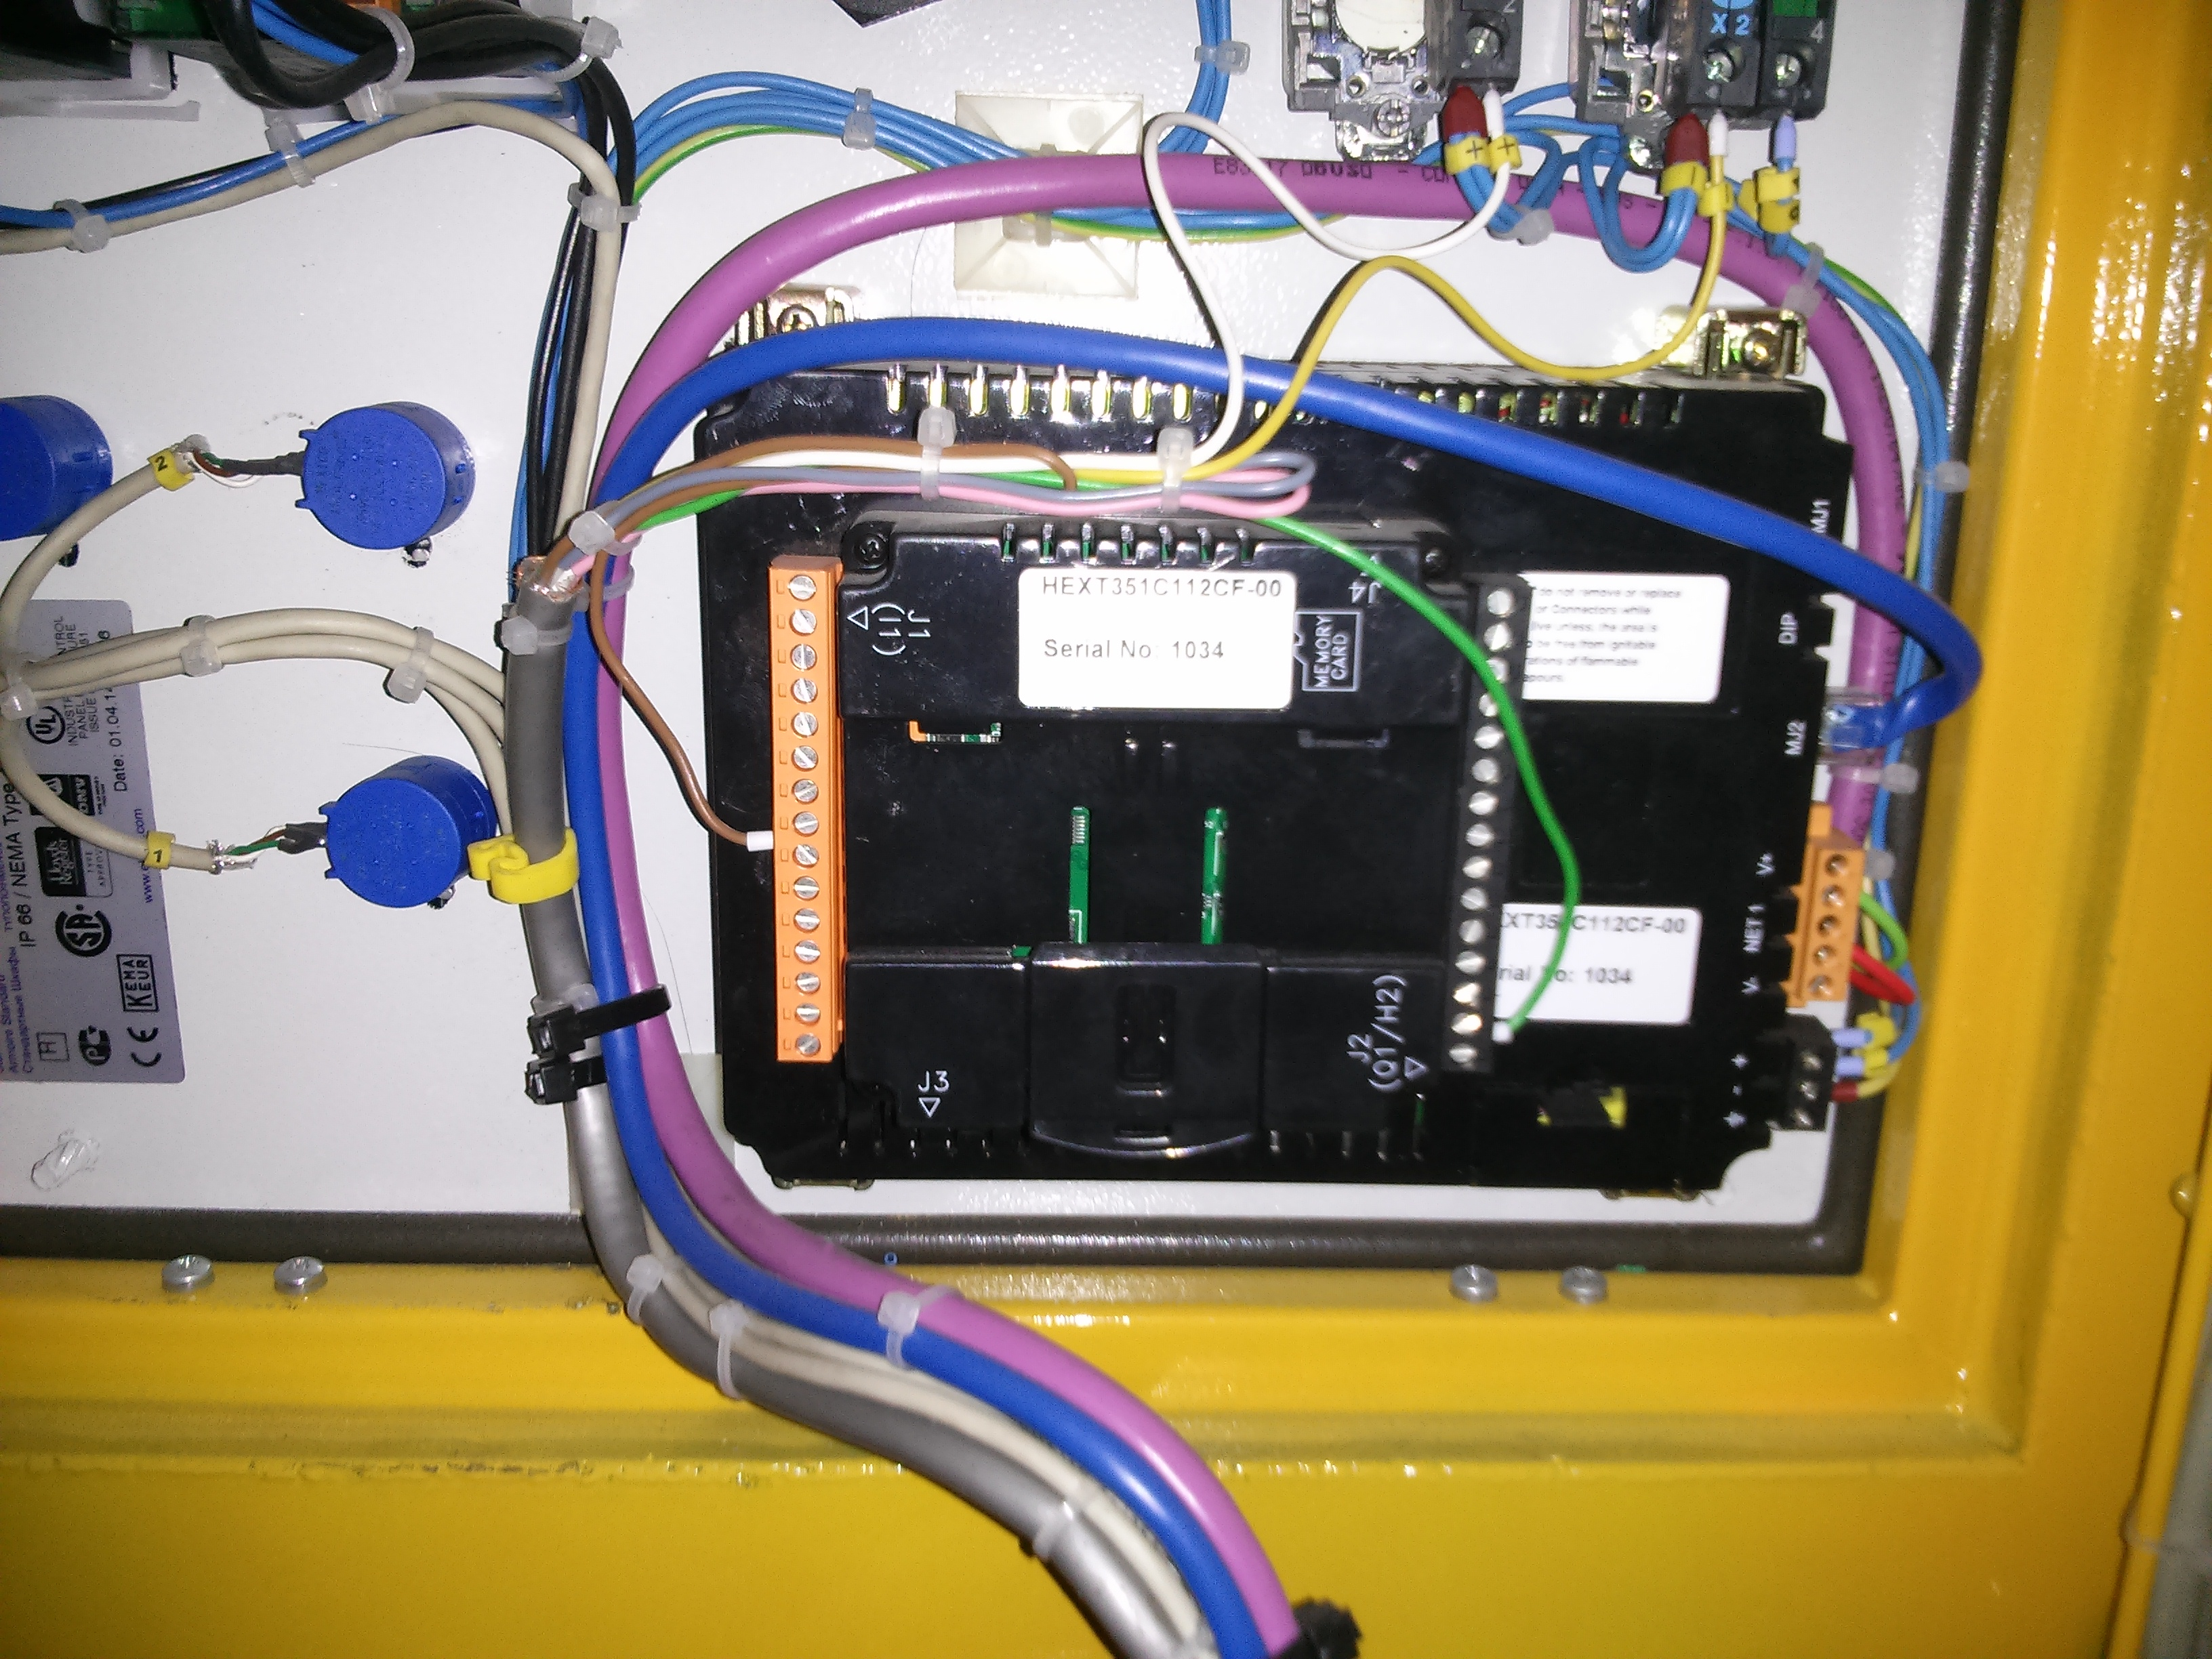
\includegraphics[width=0.4\textwidth]{images/huesca/IMG_20141216_175108.jpg}
            \caption{Pantalla HMI}
            \label{fig:hardware_HMI}
    \end{figure}

     \begin{figure}[H]
            \centering
            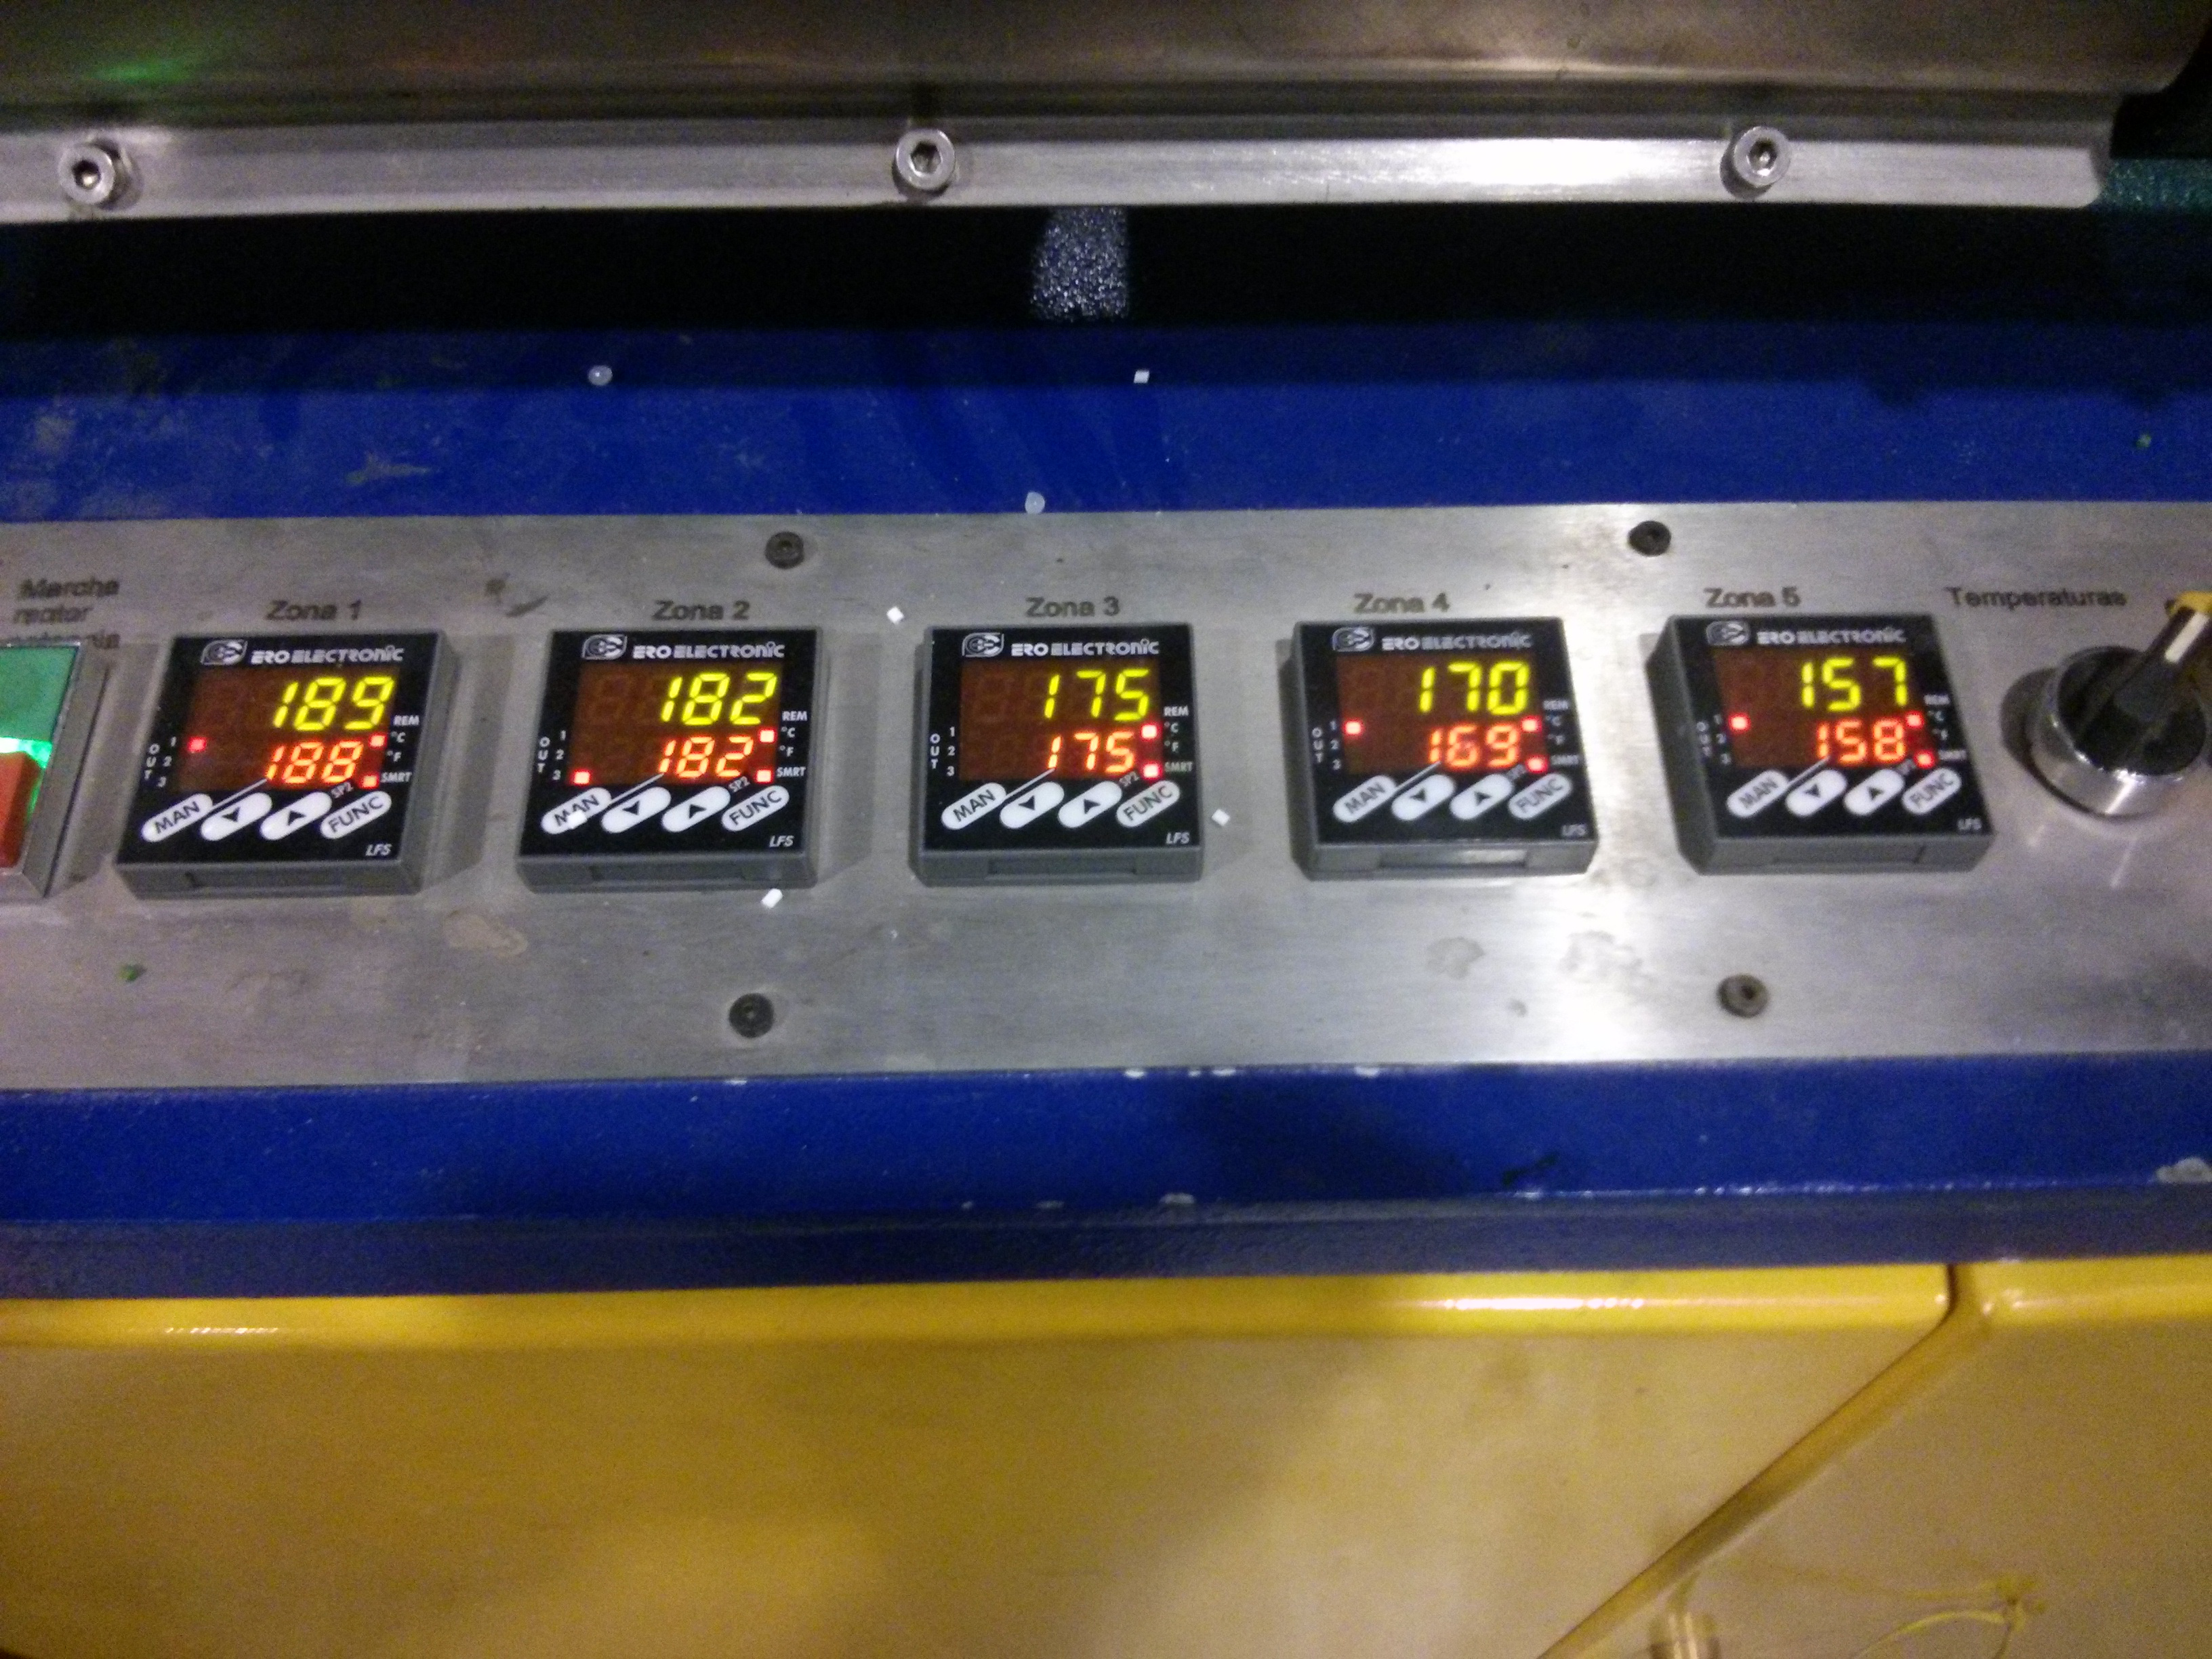
\includegraphics[width=0.4\textwidth]{images/huesca/IMG_20141216_175204.jpg}
            \caption{Sensores de temperatura}
            \label{fig:hardware_temperatura}
    \end{figure}

Buscando en internet referencias de los posibles componentes que disponemos, y con ayuda de los responsables de la fábrica, llegamos a la conclusión de que el hardware que disponemos es el siguiente:

\begin{itemize}
	\item \textbf{Reguladores temperatura Extrusora:} 5x Eroelectronic LFS
	\item \textbf{Regulador temperatura bañera:} 1x OMRON E5CC
	\item \textbf{Bobinadora: IO distribuidas: }
	\begin{itemize}

       \item {SmartStix I/O:} HE559DQM706B y HE559DI710B
       \item{HMI:} HE-XT351C112CF
        \item{Variador (control tractora):} Optidrive rrp2 ODP-24400-SP
        \item{Sensor diámetro:} conectado a módulo Adam 6066
        	\begin{itemize}
        				\item Omron ZX-GIF41 (RS232)
        				\item Omron ZX-GTC41 (Controlador)
                        \item Omron ZX-GT28S41 (sensor)
             \end{itemize}
        \item Relés: OMRON MY2IN
    \end{itemize}
\end{itemize}

Así mismo, disponemos de los datasheet y sabemos qué tipo de comunicación podemos disponer con cada uno, información necesaria para poder establecer la arquitectura del sistema.

\section{Arquitectura planteada}
\label{arquitectura}

Antes de plantear la arquitectura, deberemos establecer el protocolo de comunicaciones y el medio físio por el que irán conectados entre sí. Mirando las especificaciones de los componentes llegamos a la siguiente conclusión

\begin{table}[]

\begin{tabular}{ccc}
\hline
{\bf Dispositivo}     & {\bf Protocolo} & {\bf Medio} \\ \hline
Senores temperatura   & Modbus          & RS485       \\
Pantalla HMI          & Modbus          & RS485       \\
Adam                  & Modbus-TCP      & RS485       \\
Sensor diámetro       & -               & RS232       \\
Variador              & Modbus-TCP      & RS485       \\
Perifería distribuida & CsCAN           & Modbus      \\
Bobinadora            &                 & Cableado    \\ \hline
\end{tabular}
\centering
\caption{My caption}
\label{my-label}
\end{table}


 	\begin{figure}[H]
            \centering
            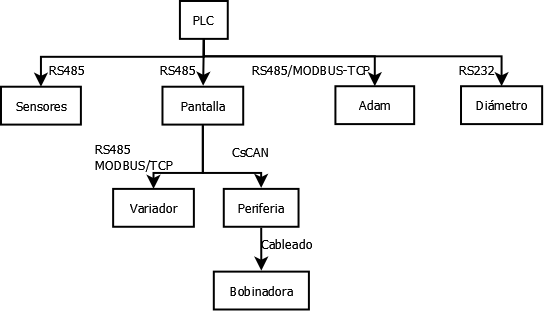
\includegraphics[width=0.6\textwidth]{images/20141229.png}
            \caption{Arquitectura propuesta}
            \label{fig:hardware_arquitectura}
    \end{figure}
